\documentclass[12pt,a4paper, openany, onecolumn]{book}

\setcounter{secnumdepth}{4}
\setcounter{tocdepth}{4}

\usepackage{color}
\usepackage{titlesec}
	\titleformat{\chapter}{\Huge\bfseries}{\filcenter\small \ CAPÍTULO \thechapter \ \newline}{7pt}{\large\bfseries\filcenter}
	\titleformat{\section}[runin]{\scshape\bf}{\thesection.}{2pt}{\color{black}}[.\quad \vspace{6pt}\\]
	\titleformat{\subsection}[runin]{\scshape\bf}{\normalsize\hspace{7pt}\thesubsection}{2pt}{\color{black}}[.\quad \vspace{6pt} \\]
	\titleformat{\subsubsection}[runin]{\scshape\bf}{\normalsize\hspace{14pt}\thesubsubsection}{2pt}{\color{black}}[.\quad \vspace{6pt} \\]
	
\usepackage[colorlinks=true, linkcolor=blue]{hyperref}
\usepackage[utf8]{inputenc}
\usepackage[spanish]{babel}
\usepackage{amsmath}
\usepackage{amsfonts}
\usepackage{amssymb}
\usepackage{makeidx}
\usepackage{graphicx}
\usepackage[left=2.5cm,right=2.5cm,top=2.5cm,bottom=2.5cm]{geometry}
\author{David}
\title{Probando}


\begin{document}
\pagestyle{plain}
\begin{titlepage}
	\begin{minipage}[t]{0.7\textwidth}
	\begin{flushleft}
		
\includegraphics[width=0.8\textwidth]{img_logos/Logo_UNFV.png}
	\end{flushleft}
	\end{minipage}
	\begin{minipage}[t]{0.2\textwidth}
	\begin{flushright}
		
\includegraphics[scale=0.3]{img_logos/Facultad.png}
	\end{flushright}
	\end{minipage}
	\par
	%\vspace{1cm}
	\centering
	\vspace{1cm}
	{\Large \bf UNIVERSIDAD NACIONAL FEDERICO VILLARREAL} \par
	\vspace{1cm}
	{\Large \bf FACULTAD DE CIENCIAS NATURALES Y MATEM\'ATICAS}\par
	\vspace{1cm}
	{\large \bf ESCUELA PROFESIONAL DE F\'ISICA} \par
	\vspace{2cm}
	{\large  T\'ITULO DE LA TESIS}\par
	\vspace{2cm}
	{\large \bf Tesis para optar el t\'itulo profesional de licenciado den f\'isica}\par
	\vspace{1cm}
	{ \bf PRESENTA:\\}
	{\large ZEVALLOS GARAY, DAVID BRANDON}\par	
	\vspace{1.5cm}
	{\bf ASESOR DE TESIS:\\}
	{\large ASESOR}\par
	\vspace{2cm}
	{\large LIMA-PER\'U}\par
	\vspace{0.5cm}
	{\large 2020}
	\end{titlepage}
%%%%%%%%%%%%%%%%%%%%%%%%%%%%%%%%%%%%%%%%%%%%%%%%%%%%%%%%%%%%%%%
%
%%%%%%%%%%%%%%%%%% DEDICATORIA
%
%%%%%%%%%%%%%%%%%%%%%%%%%%%%%%%%%%%%%%%%%%%%%%%%%%%%%%%%%%%%%%%
\newpage
\thispagestyle{empty}
	\begin{flushright}
	\begin{minipage}[t]{0.5\textwidth}
	\vspace{12cm}
	{\large \bf Dedicatoria:}\par
	A mis padres y hermana, por aguantar las noches interminables de fastidio.
	\end{minipage}
	\end{flushright}
%%%%%%%%%%%%%%%%%%%%%%%%%%%%%%%%%%%%%%%%%%%%%%%%%%%%%%%%%%%%%%%

\frontmatter

\begin{center}
{\large \bf Agradecimientos}
\end{center}


\newpage
\chapter*{\centering \large Resumen}\addcontentsline{toc}{section}{Resumen}

\newpage
\chapter*{\centering \large Abstract}\addcontentsline{toc}{section}{Abstract}

\newpage
\renewcommand{\contentsname}{Indice}
\tableofcontents
\renewcommand{\chaptername}{Capítulo}
\renewcommand{\thechapter}{\arabic{chapter}}
\renewcommand{\thesection}{\arabic{chapter}.\arabic{section}}

\newpage
\renewcommand{\listfigurename}{Indice de figuras}
\addcontentsline{toc}{section}{\listfigurename}
\listoffigures
\renewcommand{\figurename}{\textit Figura}
\renewcommand{\thefigure}{\arabic{figure}}

\newpage
\renewcommand{\listtablename}{Indice de tablas}
\addcontentsline{toc}{section}{\listtablename}
\listoftables
\renewcommand{\tablename}{\textit Tabla}
\renewcommand{\thetable}{\arabic{table}}
%%%%%%%%%%%%%%%%%%%%%%%%%%%%%%%%%%%%%%%%%%%%%%%%%%%%%%%%%%%%%%%
%
%%%%%%%%%%%%%%%%%% CAPÍTULOS
%
%%%%%%%%%%%%%%%%%%%%%%%%%%%%%%%%%%%%%%%%%%%%%%%%%%%%%%%%%%%%%%%
\mainmatter
\chapter{Introducci\'on}
Aqu\'i ir\'a la introducci\'on del trabajo.\\

\chapter{Marco teórico}
Aquí va el marco teórico.

\section{Primera sección}
Esta es la primera sección del marco teórico.
	\subsection{Subsección uno}
	Esta es la subsección
	\begin{figure}[htb]
	\centering
	
\includegraphics[scale=0.4]{Img/1.png}
	\caption{Imagen 1}
	\end{figure}
		\subsubsection{SubSubsección uno}
	\begin{figure}[htb]
	\centering
	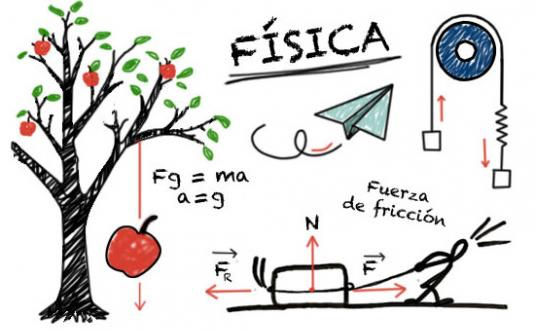
\includegraphics[scale=0.4]{Img/2.png}
	\caption{Imagen 2}
	\end{figure}
		\subsubsection{SubSubsección dos}
	\begin{figure}[htb]
	\centering
	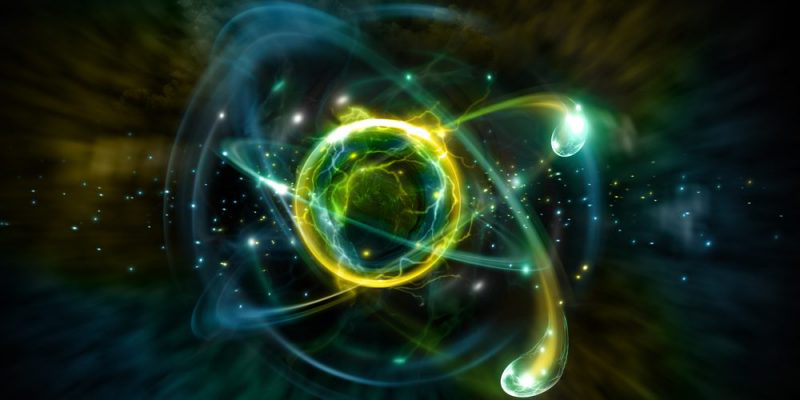
\includegraphics[scale=0.4]{Img/3.png}
	\caption{Imagen 3}
	\end{figure}
		\subsubsection{Sub-Subsección tres}
	\subsection{Subsecci\'on dos}
	Esta es la subsecci\'on dos

\section{Segunda sección}
Esta es la segunda secci\'on del marco te\'orico.
\begin{table}[htb]
\centering
\caption[Tabla 1]{Esto es un ejemplo de tabla}
\begin{tabular}{|c|c|}
\hline 
casas & mama \\ 
\hline 
tablas & papa \\ 
\hline 
\end{tabular} 
\end{table}

\chapter{Método}
Esta es la parte del método.
\section{Tercera sección}
Veremos que métodos usaremos para el trabajo final.
Es la primera sección
\section{Cuarta sección}
Esta es la segunda sección.
\chapter{Resultados}
\chapter{Discusión de resultados}
\chapter{Conclusiones}

\backmatter
\chapter{Referencias}


\chapter{Apendice}
\end{document}